\documentclass{anpet}
\usepackage[utf8]{inputenc}
\usepackage{graphicx,import}
\usepackage{booktabs}
\usepackage[english, portuguese]{babel}
\usepackage{csquotes}
\usepackage{hanging}
\usepackage{subfigure}
\usepackage{multirow}
\usepackage{siunitx}
\usepackage[hidelinks]{hyperref}
\usepackage{float}
\usepackage{mathrsfs}  
\usepackage{symbols}
\usepackage{longtable}
\sisetup{output-decimal-marker = {,}}

\addbibresource{dynamic_routing.bib} %adicione o nome do arquivo com as referencias

\title{Problemas dinâmicos de coleta e entrega com janelas de tempo: Instâncias de benchmark}
\author{Renan Artur Lopes Eccel}
\author{Rodrigo Castelan Carlson}
\affil{Universidade Federal de Santa Catarina \protect\\ Programa de Pós-Graduação em  Engenharia de Automação e Sistemas}
\date{\today}

\begin{document}

\maketitle

\begin{resumo}
Insira aqui o resumo.
\end{resumo}

\begin{abstract}
Insert the abstract here.
\end{abstract}

\section{Introdução}

\section{Problemas de interesse}
Segundo \textcite{doerner_pickup-and-delivery_2014}, \textit{Dial-a-Ride Problems} (DARP) é o nome dado ao problema de roteamento de uma frota de veículos de ocupação múltipla que ofereça um serviço de transporte porta-a-porta para os seus usuários. O serviço de transporte é compartilhado, de forma que múltiplos usuários, com diferentes origens e/ou destinos, possam ser acomodados simultaneamente em um mesmo veículo.

Portanto, o DARP padrão pode ser definido por um conjunto de pedidos de viagem, tendo cada um destes um conjunto origem e destino distintos e uma frota de veículos e rotas que devem conectar os veículos aos conjuntos de pedidos, transportando os usuários de seus locais de origem para seus destinos. O objetivo do problema é encontrar um grupo de rotas de menor custo que atenda todos os pedidos, respeitando a capacidade dos veículos, a precedência de origem destino e a qualidade do serviço \parencite{cordeau_tabu_2003}. 

\textcite{parragh_survey_2008-1} relata que esta última restrição é a principal diferença entre o DARP e o Problema de Coleta e Entrega com Janelas de Tempo (PDPTW - \textit{Pickup and Delivery Problem with Time Windows}), pois este refere-se ao transporte de mercadorias e, por conseguinte, não possui algumas das restrições de qualidade do DARP como, por exemplo, o limite superior para o tempo entre a coleta e entrega de cada pedido.
% Contudo,devido as similaridades entre estes problemas, alguns artigos analisam as instâncias de forma indistinta. Vide \cite{ropke_branch_2009}.
% TODO adicionar maior ênfase nas similaridades entre esses conjuntos de problemas

% TODO descrever os diversos tipos de DARP e mostrar qual deles será considerado para o artigo
Ademais, DARPs possuem também subdivisões dependendo das características operacionais relevantes. Existem diversas formas de catalogar as características e assim classificar os problemas \parencite{molenbruch_typology_2017, psaraftis_dynamic_2015, pillac_review_2013}, porém, este artigo usará a classificação fornecida por \textcite{ho_survey_2018}. Este artigo tratará do DARP dinâmico e determinístico, considerando uma única garagem e uma frota homogênea de veículos com restrições de capacidade. Todos os pedidos possuem janelas de tempo e restrições do tempo máximo entre a coleta e entrega.

\section{Formulação dos problemas}
\subsection{DARP definido por \textcite{cordeau_branch-and-cut_2006}}
Sendo $\numberOfRequests$ o número de usuários (pedidos) a serem servidos. O DARP pode ser definido em um grafo direcional completo $\graph(\nodes,\arcs)$, em que $\nodes = \pickupNodes \cup \deliveryNodes \cup \{\startNode, \lastNode \}$, $\pickupNodes = \{1, \ldots, \numberOfRequests\}$, e $\deliveryNodes = \{\numberOfRequests + 1, \ldots, 2\numberOfRequests\}$. Os subconjuntos $\pickupNodes$ e $\deliveryNodes$ contém nós de coleta e entrega, respectivamente, enquanto os nós $\startNode$ e $\lastNode$ representam os depósitos de origem e destino. Para cada pedido $\request$ temos associado um nó de origem $\originNode$ e um nó de destino $\destinationNode$.

Sendo $\vehiclesSet$ o conjunto de veículos. Cada veículo $\vehicle \in \vehiclesSet$ possui a capacidade de $\vehicleCapacity$, e o máximo tempo total de rota $\vehicleMaxRouteTime$. Para cada nó $\node \in \nodes$ existe um carregamento $\nodeLoad$ associado e um tempo de serviço $\nodeServiceTime$, não negativo, sendo que $\startNodeServiceTime = \lastNodeServiceTime = 0$, $\originNodeLoad = -\destinationNodeLoad$ $(\request = 1,\ldots,\numberOfRequests)$ e $\serviceTime_\startNode = \serviceTime_{\lastNode} = 0$. Uma janela de tempo $[\earliestTimeWindow_\node,\latestTimeWindow_\node]$ é também associada ao nó $\node \in \nodes$, em que $\earliestTimeWindow_\node$ e $\latestTimeWindow_\node$ representam o menor e o maior instante de tempo que o serviço deve começar no nó $\node$. Cada arco $\arc{i}{j} \in \arcs$ é associado com um custo $\arcCost{i}{j}$ e um tempo de viagem $\arcTravelTime{i}{j}$. Finalmente, denotamos por $\maxRideTime$ o tempo máximo de viagem de um usuário(pedido), e $\arrivalTime$ o instante que o pedido é feito.

\section{Dinamização de instâncias estáticas}
\textcite{ho_survey_2018} disponibiliza uma tabela catalogando instâncias de \textit{bechmark} utilizadas para o DARP. Nenhuma das apresentadas apresenta pedidos dinâmicos e somente as instâncias apresentadas por \textcite{cordeau_branch-and-cut_2006, cordeau_tabu_2003, ropke_models_2007} representam a formulação estática do problema de interesse do artigo.

 
\section{Memorando}
\begin{itemize}
    \item Segundo \textcite{parragh_survey_2008-1}, as instâncias apresentadas por \textcite{li_metaheuristic_2003} são as predominantemente usadas para avaliar a performance de algoritmos que resolvem PDPTW.

    \item Segundo \textcite{pillac_review_2013}, são escassas as instâncias de benchmark para roteamento veicular dinâmico que sejam amplamente usadas.

    \item \textcite{van_lon_measures_2016} define uma métrica para dinamismo em instâncias PDPTW e afirma que distribuições Poisson homogenias conseguem apenas criar cenários de 45 a 60 \% dinâmicos. 

   \item \textcite{van_lon_measures_2016} define uma métrica para urgência que se assemelha com o "grau de dinamismo efetivo" proposto por \textcite{larsen_partially_2002}, sendo a única diferença a normalização, em relação ao tamanho do cenário, que \textcite{larsen_partially_2002} executa. \textcite{van_lon_measures_2016} acredita que a extensão do cenário e a urgência devem ser independentes.

   \item \textcite{van_lon_towards_2015} adiciona o tamanho como uma das métricas usadas para classificar instâncias PDPTW.   
   
   \item \textcite{berbeglia_hybrid_2012} considera um tempo entre fim da janela de tempo de coleta e início da janela de entrega como sendo igual ao tempo de viagem entre os pontos de coleta e entrega.
   
   \item \textcite{schilde_metaheuristics_2011} descreve o processo de avaliar estatisticamente uma instância DARP.

\end{itemize}

\section{instâncias de Benchmark Dinâmicas}
\subsection{DARP de \textcite{berbeglia_hybrid_2012}}
\subsubsection{Primeiro conjunto \parencite{ropke_models_2007}}

\textcite{berbeglia_hybrid_2012} usa como base as instâncias estáticas propostas por \textcite{ropke_models_2007}, o qual utilizou o método proposto por \textcite{savelsbergh_drive:_1998} para a geração. Mais informações sobre estas instâncias podem ser obtidas em \textcite{cordeau_branch-and-cut_2006}.

As instâncias estáticas possuem as seguintes características:
\begin{itemize}
    \item \textbf{Horizonte de planejamento:} $\planingHorizon = 1440$ 
    \item \textbf{Geometria:} quadrado $[-10, 10]\ \times \ [-10, 10]$.
    \item \textbf{Número de pedidos:} $\numberOfRequests$, especificado na \autoref{tab:ropke_models_2007_DARP_instances_caracteristics}
    \item \textbf{Distribuição dos nós:} aleatoriamente alocados usando uma distribuição uniforme sobre a geometria. Unidades representadas por três casas decimais.
    \item \textbf{Localização dos depósitos:} $(0, 0)$, centro da geometria.
    \item \textbf{Custo de viagem entre nós:} $\arcCost{i}{j} = EuclidianDistance\arc{i}{j}, \forall \arc{i}{j} \in A$
    \item \textbf{Tempo de viagem entre nós:} $\arcTravelTime{i}{j} = \arcCost{i}{j}$
    \item \textbf{Características dos pedidos:} metade ($1,\ldots,\numberOfRequests/2$) dos pedidos possuem janela de tempo na entrega, e a outra metade ($\numberOfRequests/2 + 1, \ldots, \numberOfRequests$) possuem janela de tempo na coleta.
    \item \textbf{Número de veículos:} $|\vehiclesSet|$, especificado na \autoref{tab:ropke_models_2007_DARP_instances_caracteristics}
    \item \textbf{Capacidade do veículo:} $\vehicleCapacity=\capacity,\forall \vehicle \in \vehiclesSet$, $\capacity$ está especificado na \autoref{tab:ropke_models_2007_DARP_instances_caracteristics}
    \item \textbf{Carregamento por pedido:} 
    \begin{itemize}
        \item Para as instâncias do grupo "a" $\nodeLoad = 1, \forall \node \in \pickupNodes$
        \item Para as instâncias do grupo "b" $\nodeLoad = \uniformDistribution{1}{6}, \forall \node \in \pickupNodes$
    \end{itemize}
    \item \textbf{Tempo de serviço:} 
    \begin{itemize}
        \item $\nodeServiceTime = 3, \forall \node \in \nodes$ para as instâncias do grupo "a" 
        \item $\nodeServiceTime = \nodeLoad, \forall \node \in \nodes$ para as instâncias do grupo "b".
    \end{itemize}
    \item \textbf{Tamanho das janelas de tempo:} $\timeWindowWidth= 15$.
    \item \textbf{Geração das janelas de tempo:} A janela de tempo para o pedido $\request$ é construída selecionando aleatoriamente um $\earliestTimeWindow_\originNode$ no intervalo $[0,\planingHorizon - \arcTravelTime{\originNode}{\destinationNode}]$, e então selecionando $\latestTimeWindow_\request = \earliestTimeWindow_\originNode + \planingHorizon$, $\earliestTimeWindow_{\destinationNode} = \earliestTimeWindow_\originNode + \arcTravelTime{\originNode}{\destinationNode}$ e $\latestTimeWindow_{\destinationNode} = \earliestTimeWindow_{\destinationNode} + \planingHorizon$.
    \item \textbf{Tempo de rota máximo:} $\maxRouteTime$, especificado na \autoref{tab:ropke_models_2007_DARP_instances_caracteristics}
    \item \textbf{Tempo de viagem máximo:} $\maxRideTime$, especificado na \autoref{tab:ropke_models_2007_DARP_instances_caracteristics}
\end{itemize}

\begin{table}[H]
    \centering
    \caption{Características das instâncias DARP de \textcite{ropke_models_2007}}
    \label{tab:ropke_models_2007_DARP_instances_caracteristics}
    \begin{tabular}{lrrrrr|lrrrrr}
        \toprule
        Instância & $|\vehiclesSet|$ & $\numberOfRequests$ & $\maxRouteTime$ & $\capacity$ & $\maxRideTime$ & Instância & $|\vehiclesSet|$ & $\numberOfRequests$ & $\maxRouteTime$ & $\capacity$ & $\maxRideTime$\\
        \midrule
        a2-16 & 2 & 16 & 480 & 3 & 30 & b2-16 & 2 & 16 & 480 & 6 & 45\\
        a2-20 & 2 & 20 & 600 & 3 & 30 & b2-20 & 2 & 20 & 600 & 6 & 45\\
        a2-24 & 2 & 24 & 720 & 3 & 30 & b2-24 & 2 & 24 & 720 & 6 & 45\\
        a3-24 & 3 & 24 & 480 & 3 & 30 & b3-24 & 3 & 24 & 480 & 6 & 45\\
        a3-30 & 3 & 30 & 600 & 3 & 30 & b3-30 & 3 & 30 & 600 & 6 & 45\\
        a3-36 & 3 & 36 & 720 & 3 & 30 & b3-36 & 3 & 36 & 720 & 6 & 45\\
        a4-32 & 4 & 32 & 480 & 3 & 30 & b4-32 & 4 & 32 & 480 & 6 & 45\\
        a4-40 & 4 & 40 & 600 & 3 & 30 & b4-40 & 4 & 40 & 600 & 6 & 45\\
        a4-48 & 4 & 48 & 720 & 3 & 30 & b4-48 & 4 & 48 & 720 & 6 & 45\\
        a5-40 & 5 & 40 & 480 & 3 & 30 & b5-40 & 5 & 40 & 480 & 6 & 45\\
        a5-50 & 5 & 50 & 600 & 3 & 30 & b5-50 & 5 & 50 & 600 & 6 & 45\\
        a5-60 & 5 & 60 & 720 & 3 & 30 & b5-60 & 5 & 60 & 720 & 6 & 45\\
        a6-48 & 6 & 48 & 480 & 3 & 30 & b6-48 & 6 & 48 & 480 & 6 & 45\\
        a6-60 & 6 & 60 & 600 & 3 & 30 & b6-60 & 6 & 60 & 600 & 6 & 45\\
        a6-72 & 6 & 72 & 720 & 3 & 30 & b6-72 & 6 & 72 & 720 & 6 & 45\\
        a7-56 & 7 & 56 & 480 & 3 & 30 & b7-56 & 7 & 56 & 480 & 6 & 45\\
        a7-70 & 7 & 70 & 600 & 3 & 30 & b7-70 & 7 & 70 & 600 & 6 & 45\\
        a7-84 & 7 & 84 & 720 & 3 & 30 & b7-84 & 7 & 84 & 720 & 6 & 45\\
        a8-64 & 8 & 64 & 480 & 3 & 30 & b8-64 & 8 & 64 & 480 & 6 & 45\\
        a8-80 & 8 & 80 & 600 & 3 & 30 & b8-80 & 8 & 80 & 600 & 6 & 45\\
        a8-96 & 8 & 96 & 720 & 3 & 30 & b8-96 & 8 & 96 & 720 & 6 & 45\\
        \bottomrule
    \end{tabular}
\end{table}

\subsubsection{Segundo conjunto \parencite{cordeau_tabu_2003}}
20 instâncias, com número de pedidos variando entre 24 e 144.

As instâncias estáticas possuem as seguintes características:
\begin{itemize}
    \item \textbf{Horizonte de planejamento:} $\planingHorizon=1440$
    \item \textbf{Geometria:} quadrado $[-10, 10]\ \times \ [-10, 10]$.
    \item \textbf{Número de pedidos:} $\numberOfRequests$, especificado na \autoref{tab:cordeau_tabu_2003_DARP_intances_characteristics}
    \item \textbf{Distribuição dos nós:} Gerados usando o procedimento descrito em \textcite{cordeau_tabu_1997}, que cria grupos de nós próximos a pontos pré-determinados.
    \item \textbf{Localização dos depósitos:} média dos pontos pré-determinados.
    \item \textbf{Custo de viagem entre nós:} $\arcCost{i}{j} = EuclidianDistance\arc{i}{j}, \forall \arc{i}{j} \in \arcs$
    \item \textbf{Tempo de viagem entre nós:} $\arcTravelTime{i}{j} = \arcCost{i}{j}$
    \item \textbf{Características dos pedidos:} metade ($1,\ldots,\numberOfRequests/2$) dos pedidos possuem janela de tempo na entrega, e a outra metade ($\numberOfRequests/2 + 1, \ldots, \numberOfRequests$) possuem janela de tempo na coleta.
    \item \textbf{Número de veículos:} $|\vehiclesSet|$, especificado na \autoref{tab:cordeau_tabu_2003_DARP_intances_characteristics}
    \item \textbf{Capacidade do veículo:} $\vehicleCapacity=6,\forall \vehicle \in \vehiclesSet$
    \item \textbf{Carregamento por pedido:} $\requestLoad = 1$
    \item \textbf{Tempo de serviço:} $\nodeServiceTime = 10$ 
    \item \textbf{Tamanho das janelas de tempo:} 
    \begin{itemize}
        \item Para o grupo (a): $\timeWindowWidth = 30$
        \item Para o grupo (b): $\timeWindowWidth = 60$
    \end{itemize}
    \item \textbf{Geração das janelas de tempo:}     \begin{itemize}
        \item Para o grupo (a) janelas de tempo restritas foram geradas $\earliestTimeWindow_\node = \uniformDistribution{60}{480}$ e $\latestTimeWindow_\node = \uniformDistribution{\earliestTimeWindow_\node + 15}{ \earliestTimeWindow_\node + 45}$
        \item Para o grupo (b) janelas de tempo relaxadas foram geradas: $\earliestTimeWindow_\node = \uniformDistribution{60}{480}$ e $\latestTimeWindow_\node = \uniformDistribution{\earliestTimeWindow_\node + 30}{\earliestTimeWindow_\node + 90}$
    \end{itemize}
    
    \item \textbf{Tempo de rota máximo:} $\maxRouteTime = 480$
    \item \textbf{Tempo de viagem máximo:}$\maxRideTime = 90$
\end{itemize}

\begin{table}[H]
    \centering
    \caption{Características das instâncias DARP de \textcite{cordeau_tabu_2003}}
    \label{tab:cordeau_tabu_2003_DARP_intances_characteristics}
    \begin{tabular}{lrr|lrr}
        \toprule  
        Instância & $\numberOfRequests$ & $|\vehiclesSet|$ & Instância & $\numberOfRequests$ & $|\vehiclesSet|$\\
        \midrule
        R1a  &  24 &  3 & R1b  &  24 &  3\\
        R2a  &  48 &  5 & R2b  &  48 &  5\\
        R3a  &  72 &  7 & R3b  &  72 &  7\\
        R4a  &  96 &  9 & R4b  &  96 &  9\\
        R5a  & 120 & 11 & R5b  & 120 & 11\\
        R6a  & 144 & 13 & R6b  & 144 & 13\\
        R7a  &  36 &  4 & R7b  &  36 &  4\\
        R8a  &  72 &  6 & R8b  &  72 &  6\\
        R9a  & 108 &  8 & R9b  & 108 &  8\\
        R10a & 144 & 10 & R10b & 144 & 10\\
        \bottomrule
    \end{tabular}
\end{table}

\textcite{berbeglia_hybrid_2012} torna estas instâncias dinâmicas através do seguinte método. Denota-se que as foram usadas apenas as instâncias com no mínimo 40 pedidos:

Define-se um par de parâmetros $(\staticPercentage,\maneuverTime)$, em que $\staticPercentage \in [0, 1]$ e define a porcentagem de pedidos conhecidos no início do horizonte de tempo. Se $\staticPercentage = 0$ o problema é totalmente dinâmico, similarmente, se $\staticPercentage = 1$ o problema é estático e todos os pedidos são conhecidos a priori.  

Dado um pedido $\request$, o valor $\requestLatestArrivalTime$ consiste em um limite superior para o instante que o pedido deve ser conhecido para que seja possível servi-lo. O valor $\maneuverTime$ indica quão tempo antes de $\requestLatestArrivalTime$ o pedido é conhecido.

\begin{equation}
    \requestLatestArrivalTime = \min\{\latestTimeWindow_{\originNode},\ \latestTimeWindow_{\destinationNode}  - \arcTravelTime{\originNode}{\destinationNode} - \serviceTime_{\request}\}
    \label{eq:berbeglia_hybrid_2012_requestLatestArrivalTime}
\end{equation}

\begin{equation}
    \requestArrivalTime = \requestLatestArrivalTime - \maneuverTime
    \label{eq:berbeglia_hybrid_2012_requestArrivalTime}
\end{equation}

No artigo os parâmetros $\staticPercentage = 0,25$ e $\maneuverTime = 60$ para a dinamização dos subconjuntos $a$ e $b$ das instâncias apresentadas em \textcite{ropke_models_2007}. Já o conjunto de instâncias pertencentes à \textcite{cordeau_tabu_2003}, cujos rótulos iniciam com "pr", foi transformado em um conjunto de instâncias dinâmicas usando os parâmetros $\staticPercentage = 0,25$ e $\maneuverTime =\uniformDistribution{60}{240}$. Por último, dos 200 pedidos baseados em dados reais apresentados por \textcite{cordeau_tabu_2003}, foram criadas 12 diferentes instâncias, com valores diferentes para as janelas de tempo e para o número total de pedidos. Estas instâncias foram transformadas em dinâmicas através do método apresentado e usando os parâmetros $\staticPercentage = 0,25$ e $\maneuverTime =\uniformDistribution{60}{240}$.

\subsection{Instâncias realísticas de DARP propostas por \textcite{schilde_metaheuristics_2011}}

Neste artigo, os autores propõe a criação de instâncias realísticas baseadas em dados fornecidos pela Cruz Vermelha Austríaca durante o ano de 2004 na cidade de Granz. No total foram fornecidos dados de 125.035 pedidos. O restante da seção apresenta um resumo da análise de dados executada por \textcite{kritzinger_warteschlangentheorie_2008}.

A primeira observação tirada dos dados foi que metade dos pedidos eram conhecidos pela manhã (estáticos). Os outros eram conhecidos durante a operação (dinâmicos). Os tempos entre pedidos foram calculados, filtrados e separados em segmentos de 1 hora. Para cada segmento intervalos de 10 minutos foram analisados, contabilizando o número de tempo entre pedidos que se encaixam em cada um deles. A análise indicou uma distribuição exponencial. Essa suposição foi testada usando testes qui-quadrados. A hipótese nula foi que os dados era exponencialmente distribuídos com uma densidade contínua $f(x) = \lambda e^{-\lambda x}, \forall \lambda>0$ e um valor esperado $E(X) = 1/\lambda$.

O parâmetro $\lambda$ foi determinado usando usando uma estimativa de máxima verossimilhança do recíproco do valor médio da amostra. O teste qui-quadrado retornou resultados positivos para aproximadamente 70\% de todos os casos (não rejeita a hipótese nula). Para o tempo entre a ocorrência do pedido e o último instante possível de chegada no hospital, resultados sugestem uma distribuição gama com densidade contínua $f(x) = \lambda/\Gamma(\alpha)(\lambda x)^{\alpha - 2}e^{-\lambda x}$, através do qual $\alpha, \lambda > 0$, o valor esperado $E(X)=\alpha/\lambda$, e a variância é $Var(X) = \alpha/\lambda^2$. Os valores para $\alpha$ e $\lambda$ foram estimados usando o método dos momentos generalizados, o que provou fornecer uma boa estimativa.

\subsection{Instâncias DPDPTW propostas por \textcite{van_lon_measures_2016}}
Neste artigo os autores propões uma nova definição das métricas de dinamismo e urgência em uma instância do PDPTW (Pickup and Delivery Problem with Time Windows). Como premissa, os autores consideram que estas variáveis devem ser relacionadas apenas ao problema, e portanto, o algoritmo usado para solução não deve influenciar em seus valores. Entrentanto, estas métricas devem colaborar com uma correta análise de algorítmos para uma dada instância. Além disso, as medidas devem ser interdependentes, não havendo coorelação entre suas definições.

\subsubsection{Dinamismo}
Define-se primeiramente que grau de dinamismo é dado através da continuidade de mudança. Um cenário muito dinâmico é caracterizado por mudanças contínuas, em oposição a um cenário pouco dinâmico, onde mudanças ocorrem ocasionalmente. A figura abaixo demonstra, através de exemplos, as indicações anteriores. Também define-se uma mudança como um evento que adiciona informações ao problema. Um pedido de viagem pode ser considerado um evento deste tipo.

\begin{figure}[H]
    \begin{center}
        \makebox[\textwidth]{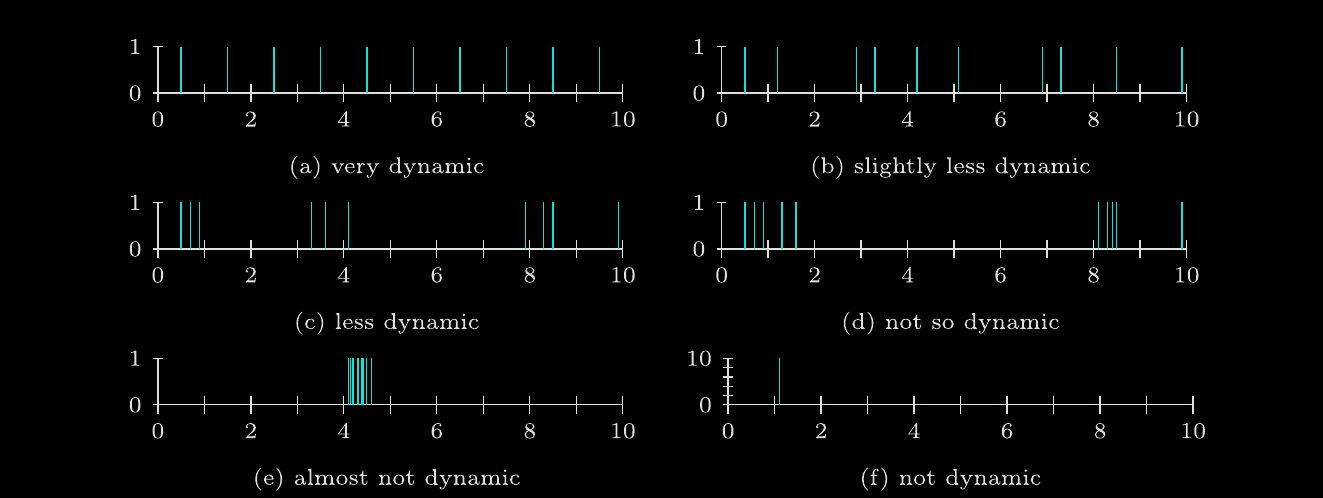
\includegraphics[width=\paperwidth]{fig/dinamismo.png}}
        \caption{Dinamismo}
        \label{fig:van_lon_measures_2016_dynamism}
    \end{center} 
\end{figure}

Defini-se $\intervalsBetweenArrivals$ como uma lista de intervalos de chegada de pedidos, através da equação a seguir:

\begin{equation}
    \intervalsBetweenArrivals := \{\intervalBetweenArrivals_0,\intervalBetweenArrivals_1,\ldots, \intervalBetweenArrivals_{\numberOfRequests-2}\} = \{\arrivalTime_j - \arrivalTime_i \mid j = i + 1 \wedge \forall i, j \in \pickupNodes\}
    \label{eq:van_lon_measures_2016_intervalsBetweenArrivals}
\end{equation}

\begin{equation}
    |\intervalsBetweenArrivals| := |\pickupNodes| - 1
    \label{eq:van_lon_measures_2016_intervalsBetweenArrivalsSize}
\end{equation}

Define-se $\perfectInterval$ como sendo o perfeito intervalo de chegada:

\begin{equation}
    \perfectInterval := \frac{H}{|\pickupNodes|}
    \label{eq:van_lon_measures_2016_perfectInterval}
\end{equation}

Portanto, calcula-se o desvio entre os intervalos de chegada contidos em $\intervalsBetweenArrivals$ com o intervalo perfeito:

\begin{equation}
    \deviationFromPerfectInterval_i :=
        \begin{cases}
            \perfectInterval - \intervalBetweenArrivals_i & \text{if $i = 0$ and $\intervalBetweenArrivals_i < \perfectInterval$} \\
            
            \perfectInterval - \intervalBetweenArrivals_i + \frac{\perfectInterval-\intervalBetweenArrivals_i}{\perfectInterval} \cdot \deviationFromPerfectInterval_{i-1} & \text{if $i > 0$ and $\intervalBetweenArrivals_i < \perfectInterval$} \\
            
            0 & \text{otherwise}
        \end{cases}
    \label{eq:van_lon_measures_2016_deviationFromPerfectInterval}
\end{equation}

Sendo que o termo $\frac{\perfectInterval-\intervalBetweenArrivals_i}{\perfectInterval} \cdot \deviationFromPerfectInterval_{i-1}$ serve para penalizar, de forma recursiva, aglutinação de eventos em pequenos períodos de tempo(\textit{bursts}). \textbf{Não seria isso um valor arbitrário?}

Consequentemente, o desvio total do cenário pode ser definido pela :
\begin{equation}
    \sum_{i=0}^{|\intervalsBetweenArrivals|} \deviationFromPerfectInterval_i
    \label{eq:van_lon_measures_2016_totalDeviationFromPerfectInterval}
\end{equation}

Entretanto, se faz necessária a normalização do desvio total do cenário. Para isso, define-se o maior valor possível:

\begin{equation}
    \sum_{i=0}^{|\intervalsBetweenArrivals|} \overline{\deviationFromPerfectInterval}_i
    \label{eq:van_lon_measures_2016_bigestTotalDeviationFromPerfectInterval}
\end{equation}

Em que:

\begin{equation}
    \overline{\deviationFromPerfectInterval}_i := \perfectInterval + 
        \begin{cases}
            \frac{\perfectInterval - \intervalBetweenArrivals_i} {\perfectInterval} \cdot \deviationFromPerfectInterval_{i-1} & \text{if $i>0$ and $\intervalBetweenArrivals_i < \perfectInterval$} \\
            0 & \text{otherwise}
        \end{cases}
    \label{eq:van_lon_measures_2016_bigestDeviationFromPerfectInterval}    
\end{equation}

combinando as Equações \ref{eq:van_lon_measures_2016_totalDeviationFromPerfectInterval} e \ref{eq:van_lon_measures_2016_bigestTotalDeviationFromPerfectInterval}, define-se dinamismo como:

\begin{equation}
    dynamism := 1 - \frac{deviation}{max\text{ }deviation} = 1 - \frac{\sum_{i=0}^{|\intervalsBetweenArrivals|} \deviationFromPerfectInterval_i}{\sum_{i=0}^{|\intervalsBetweenArrivals|} \overline{\deviationFromPerfectInterval}_i}
    \label{eq:van_lon_measures_2016_dynamism}
\end{equation}

\subsubsection{Urgência} 

Urgência é o tempo de reação disponível para atender a um pedido. Pode ser expressa através de unidades de tempo e definida através da diferença entre o instante de chegada do pedido e o último instante referente a janela de tempo da coleta. A figura abaixo exemplifica o caso.

\begin{figure}[H]
    \begin{center}
        \makebox[\textwidth]{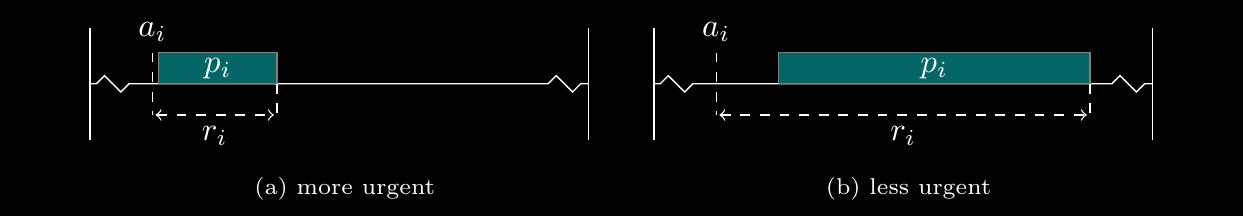
\includegraphics[width=\paperwidth]{fig/urgencia.png}}
        \caption{Urgência}
        \label{fig:van_lon_measures_2016_urgency}
    \end{center} 
\end{figure}

Baseando-se na \autoref{fig:van_lon_measures_2016_urgency}, define-se urgência para um evento através da \autoref{eq:van_lon_measures_2016_urgency}:

\begin{equation}
    \urgency_\request := \earliestTimeWindow_\request - \arrivalTime_\request
    \label{eq:van_lon_measures_2016_urgency}
\end{equation}

Urgência é o tempo de reação expresso em unidades de tempo. Para obter uma indicação da urgência de um cenário completo, pode-se computar a média e o desvio padrão das urgências. Esta definição está similar ao "grau de dinamismo efetivo" proposta por \textcite{larsen_partially_2002}, sendo a única diferença a normalização, em relação ao tamanho do cenário, que Larsen executa. Van Lon et al. acredita que a extensão do cenário e a urgência devem ser independentes.

\subsubsection{Geração de Instâncias}

Von Lon et al. também propôs um método para geração de instâncias DPDPTW com diferentes valores de dinamismo e urgência. Este método usa um conjunto de 11 níveis de dinamismo (0-100 por cento com acréscimos de 10 por cento) e 10 níveis de urgência (0-45 minutos com acréscimos de 5 minutos). Isto resulta em 110 diferentes configurações. Ao total foram produzidas 20 instâncias distintas de cada uma das possíveis configurações, resultando em 2200 cenários. 

Para a distribuição dos eventos dentro do horizonte dos cenários Van Lon et al. usou 4 distribuições distintas, cada qual para um intervalo especifico de dinamismo.

\begin{table}[H]
    \caption{Distribuições utilizadas para a geração de instantes de pedidos}
    \label{tab:van_lon_measures_2016_distributions}
    \centering
    \begin{tabular}{lr}
        \text{Poison homogênea}             & 50-55  \% \\
        \text{Poison não homogênea}         &  0-45  \% \\
        \text{Distribuição normal truncada} & 60-65  \% \\
        \text{Distribuição uniforme}        & 70-100 \% \\
    \end{tabular}
\end{table}


\subsection{Instâncias DPDPTW propostas por \textcite{pureza_waiting_2008}}

As instâncias foram geradas através da dinamização das instâncias estáticas com 100, 200 e 400 nós (50, 100 e 200 pedidos) propostas por \textcite{li_metaheuristic_2003}. Seguindo a classificação de \textcite{solomon_algorithms_1987},  \textcite{li_metaheuristic_2003} organizaram as instâncias em seis classes, denotadas por LC1, LC2, LR1, LR2, LRC1 e LRC2, indicando as respectivas distribuições espaciais dos nós e o tamanho dos horizontes de planejamento. Nos conjuntos LC1 e LC2 os nós são agrupados, enquanto LR1 e LR2 possuem nós aleatoriamente distribuídos. Os nós presentes nas instâncias LCR1 e LCR2 são parcialmente agrupados e parcialmente distribuídos aleatoriamente. As instancias LC1, LR1 e LRC1 possuem um horizonte de planejamento curto, enquanto LC2, LR2 e LRC1 possuem um horizonte longo.

As instâncias estáticas possuem as seguintes características:
\begin{itemize}
    \item \textbf{Horizonte de planejamento:} $\planingHorizon$ definido na tabela %TODO
    \item \textbf{Geometria:} quadrado $[0, 100]\ \times \ [0, 100]$.
    \item \textbf{Número de pedidos:} $\numberOfRequests$, especificado na tabela %TODO
    \item \textbf{Distribuição dos nós:} 
    \begin{itemize}
        \item Para as instancias LC: Gerados de forma aglutinada (\textit{clustered})
        \item Para as instâncias LR: Gerados de forma aleatória sobre uma distribuição uniforme
        \item Para as instâncias LRC: Um conjunto misto de nós uniformemente distribuídos e aglutinados
    \end{itemize}
    \item \textbf{Localização do depósito:} Diferente para cada instância.
    \item \textbf{Custo de viagem entre nós:} $\arcCost{i}{j} = EuclidianDistance\arc{i}{j}, \forall \arc{i}{j} \in \arcs$
    \item \textbf{Tempo de viagem entre nós:} $\arcTravelTime{i}{j} = \arcCost{i}{j}$
    \item \textbf{Características dos pedidos:} 
    \item \textbf{Número de veículos:} $|\vehiclesSet| = 25$
    \item \textbf{Capacidade do veículo:} $\vehicleCapacity$, especificado na tabela
    \item \textbf{Carregamento por pedido:} $\nodeLoad$, especifico para cada pedido, variando entre 3 e 36
    \item \textbf{Tempo de serviço:} $\nodeServiceTime = 90$ 
    \item \textbf{Tamanho das janelas de tempo:} $\timeWindowWidth = 2 \times \normalDistribution{\mu}{\sigma^2}$
    \item \textbf{Geração das janelas de tempo:} 
    \begin{itemize}
        \item Para as instancias LR e LRC o ponto central da janela de tempo foi criado usando: $\midTimeWindow_\node =\uniformDistribution{e_0 + t_{0,i}}{l_0 - t_{i,0} - d_i}$
        \item Para as instancias LC o ponto central da janela de tempo foi criado usando primeiramente uma rotina 3-opt (\parencite{lin_computer_1965}) em cada grupo para criar rotas e produzir programações selecionando uma orientação para cada grupo. As restrições da janela de tempo são geradas escolhendo o centro delas $\midTimeWindow$ como o instante de chegada em cada nó
    \end{itemize}
    \item \textbf{Tempo de rota máximo:} $\maxRouteTime = \planingHorizon$, especificado na tabela
    \item \textbf{Tempo de viagem máximo:} $\maxRideTime = \maxRouteTime$. Por ser um PDPTW, o tempo de viagem é limitado pelo tempo de rota.
\end{itemize}

\begin{table}[H]
    \centering
    \caption{Características das instâncias PDPTW de \textcite{li_metaheuristic_2003}}
    \label{tab:li_metaheuristics_2003_PDPTW_instances_characteristics}
    \begin{tabular}{lrrr|lrrr|lrrr}
        \toprule  
        Instância & $\planingHorizon$ & $\numberOfRequests$ & $\vehicleCapacity$ & Instância & $\planingHorizon$ & $\numberOfRequests$ & $\vehicleCapacity$ & Instância & $\planingHorizon$ & $\numberOfRequests$ & $\vehicleCapacity$ \\ 
        \midrule
        LC101      & 1236 &  53 & 200 & LR101      &  230 &  53 &  200 & LRC101      &  240 &  53 &  200\\
        LC102      & 1236 &  53 & 200 & LR102      &  230 &  55 &  200 & LRC102      &  240 &  53 &  200\\
        LC103      & 1236 &  52 & 200 & LR103      &  230 &  52 &  200 & LRC103      &  240 &  53 &  200\\
        LC104      & 1236 &  53 & 200 & LR104      &  230 &  52 &  200 & LRC104      &  240 &  54 &  200\\
        LC105      & 1236 &  53 & 200 & LR105      &  230 &  53 &  200 & LRC105      &  240 &  54 &  200\\
        LC106      & 1236 &  53 & 200 & LR106      &  230 &  52 &  200 & LRC106      &  240 &  53 &  200\\
        LC107      & 1236 &  53 & 200 & LR107      &  230 &  52 &  200 & LRC107      &  240 &  53 &  200\\
        LC108      & 1236 &  53 & 200 & LR108      &  230 &  50 &  200 & LRC108      &  240 &  52 &  200\\
        LC109      & 1236 &  53 & 200 & LR109      &  230 &  53 &  200 &             &      &     &     \\ 
                   &      &     &     & LR110      &  230 &  52 &  200 &             &      &     &     \\ 
                   &      &     &     & LR111      &  230 &  54 &  200 &             &      &     &     \\
                   &      &     &     & LR112      &  230 &  53 &  200 &             &      &     &     \\
                   &      &     &     &            &      &     &      &             &      &     &     \\
        LC201      & 3390 &  51 & 700 & LR201      & 1000 &  51 & 1000 & LRC201      & 1000 &  51 & 1000\\
        LC202      & 3390 &  51 & 700 & LR202      & 1000 &  50 & 1000 & LRC202      & 1000 &  51 & 1000\\
        LC203      & 3390 &  51 & 700 & LR203      & 1000 &  51 & 1000 & LRC203      & 1000 &  51 & 1000\\
        LC204      & 3390 &  51 & 700 & LR204      & 1000 &  50 & 1000 & LRC204      & 1000 &  51 & 1000\\
        LC205      & 3390 &  51 & 700 & LR205      & 1000 &  51 & 1000 & LRC205      & 1000 &  51 & 1000\\
        LC206      & 3390 &  51 & 700 & LR206      & 1000 &  50 & 1000 & LRC206      & 1000 &  51 & 1000\\
        LC207      & 3390 &  51 & 700 & LR207      & 1000 &  51 & 1000 & LRC207      & 1000 &  51 & 1000\\
        LC208      & 3390 &  51 & 700 & LR208      & 1000 &  50 & 1000 & LRC208      & 1000 &  51 & 1000\\
                   &      &     &     & LR209      & 1000 &  51 & 1000 &             &      &     &     \\
                   &      &     &     & LR210      & 1000 &  51 & 1000 &             &      &     &     \\
                   &      &     &     & LR211      & 1000 &  50 & 1000 &             &      &     &     \\
        \midrule
        LC1\_2\_1  & 1351 & 106 & 200 & LR1\_2\_1  &  634 & 105 &  200 & LRC1\_2\_1  &  634 & 106 &  200\\
        LC1\_2\_2  & 1351 & 105 & 200 & LR1\_2\_2  &  634 & 105 &  200 & LRC1\_2\_2  &  634 & 103 &  200\\
        LC1\_2\_3  & 1351 & 103 & 200 & LR1\_2\_3  &  634 & 104 &  200 & LRC1\_2\_3  &  634 & 105 &  200\\
        LC1\_2\_4  & 1351 & 105 & 200 & LR1\_2\_4  &  634 & 105 &  200 & LRC1\_2\_4  &  634 & 106 &  200\\
        LC1\_2\_5  & 1351 & 107 & 200 & LR1\_2\_5  &  634 & 106 &  200 & LRC1\_2\_5  &  634 & 107 &  200\\
        LC1\_2\_6  & 1351 & 107 & 200 & LR1\_2\_6  &  634 & 107 &  200 & LRC1\_2\_6  &  634 & 105 &  200\\
        LC1\_2\_7  & 1351 & 107 & 200 & LR1\_2\_7  &  634 & 103 &  200 & LRC1\_2\_7  &  634 & 106 &  200\\
        LC1\_2\_8  & 1351 & 105 & 200 & LR1\_2\_8  &  634 & 103 &  200 & LRC1\_2\_8  &  634 & 104 &  200\\
        LC1\_2\_9  & 1351 & 105 & 200 & LR1\_2\_9  &  634 & 105 &  200 & LRC1\_2\_9  &  634 & 104 &  200\\
        LC1\_2\_10 & 1351 & 104 & 200 & LR1\_2\_10 &  634 & 104 &  200 & LRC1\_2\_10 &  634 & 105 &  200\\
                   &      &     &     &            &      &     &      &             &      &     &     \\
        LC2\_2\_1  & 3598 & 102 & 700 & LR2\_2\_1  & 2535 & 101 & 1000 & LRC2\_2\_1  & 2535 & 101 & 1000\\
        LC2\_2\_2  & 3598 & 102 & 700 & LR2\_2\_2  & 2535 & 101 & 1000 & LRC2\_2\_2  & 2535 & 102 & 1000\\
        LC2\_2\_3  & 3598 & 101 & 700 & LR2\_2\_3  & 2535 & 101 & 1000 & LRC2\_2\_3  & 2535 & 101 & 1000\\
        LC2\_2\_4  & 3598 & 102 & 700 & LR2\_2\_4  & 2535 & 101 & 1000 & LRC2\_2\_4  & 2535 & 101 & 1000\\
        LC2\_2\_5  & 3598 & 101 & 700 & LR2\_2\_5  & 2535 & 102 & 1000 & LRC2\_2\_5  & 2535 & 101 & 1000\\
        LC2\_2\_6  & 3598 & 101 & 700 & LR2\_2\_6  & 2535 & 100 & 1000 & LRC2\_2\_6  & 2535 & 101 & 1000\\
        LC2\_2\_7  & 3598 & 101 & 700 & LR2\_2\_7  & 2535 & 101 & 1000 & LRC2\_2\_7  & 2535 & 101 & 1000\\
        LC2\_2\_8  & 3598 & 102 & 700 & LR2\_2\_8  & 2535 & 100 & 1000 & LRC2\_2\_8  & 2535 & 101 & 1000\\
        LC2\_2\_9  & 3598 & 101 & 700 & LR2\_2\_9  & 2535 & 100 & 1000 & LRC2\_2\_9  & 2535 & 101 & 1000\\
        LC2\_2\_10 & 3598 & 101 & 700 & LR2\_2\_10 & 2535 & 101 & 1000 & LRC2\_2\_10 & 2535 & 101 & 1000\\
        \midrule
        LC1\_4\_1  & 1501 & 211 & 200 & LR1\_4\_1  &  804 & 208 &  200 & LRC1\_4\_1  &  765 & 208 &  200\\
        LC1\_4\_2  & 1501 & 211 & 200 & LR1\_4\_2  &  804 & 209 &  200 & LRC1\_4\_2  &  765 & 209 &  200\\
        LC1\_4\_3  & 1501 & 210 & 200 & LR1\_4\_3  &  804 & 208 &  200 & LRC1\_4\_3  &  765 & 206 &  200\\
        LC1\_4\_4  & 1501 & 208 & 200 & LR1\_4\_4  &  804 & 210 &  200 & LRC1\_4\_4  &  765 & 207 &  200\\
        LC1\_4\_5  & 1501 & 211 & 200 & LR1\_4\_5  &  804 & 206 &  200 & LRC1\_4\_5  &  765 & 207 &  200\\
        LC1\_4\_6  & 1501 & 211 & 200 & LR1\_4\_6  &  804 & 211 &  200 & LRC1\_4\_6  &  765 & 208 &  200\\
        LC1\_4\_7  & 1501 & 211 & 200 & LR1\_4\_7  &  804 & 208 &  200 & LRC1\_4\_7  &  765 & 211 &  200\\
        LC1\_4\_8  & 1501 & 208 & 200 & LR1\_4\_8  &  804 & 211 &  200 & LRC1\_4\_8  &  765 & 208 &  200\\
        LC1\_4\_9  & 1501 & 209 & 200 & LR1\_4\_9  &  804 & 209 &  200 & LRC1\_4\_9  &  765 & 209 &  200\\
        LC1\_4\_10 & 1501 & 208 & 200 & LR1\_4\_10 &  804 & 209 &  200 & LRC1\_4\_10 &  765 & 209 &  200\\
                   &      &     &     &            &      &     &      &             &      &     &     \\
        LC2\_4\_1  & 3693 & 203 & 700 & LR2\_4\_1  & 3213 & 201 & 1000 & LRC2\_4\_1  & 3060 & 203 & 1000\\
        LC2\_4\_2  & 3693 & 202 & 700 & LR2\_4\_2  & 3213 & 201 & 1000 & LRC2\_4\_2  & 3060 & 203 & 1000\\
        LC2\_4\_3  & 3693 & 203 & 700 & LR2\_4\_3  & 3213 & 202 & 1000 & LRC2\_4\_3  & 3060 & 201 & 1000\\
        LC2\_4\_4  & 3693 & 203 & 700 & LR2\_4\_4  & 3213 & 202 & 1000 & LRC2\_4\_4  & 3060 & 203 & 1000\\
        LC2\_4\_5  & 3693 & 203 & 700 & LR2\_4\_5  & 3213 & 202 & 1000 & LRC2\_4\_5  & 3060 & 203 & 1000\\
        LC2\_4\_6  & 3693 & 203 & 700 & LR2\_4\_6  & 3213 & 201 & 1000 & LRC2\_4\_6  & 3060 & 203 & 1000\\
        LC2\_4\_7  & 3693 & 204 & 700 & LR2\_4\_7  & 3213 & 203 & 1000 & LRC2\_4\_7  & 3060 & 202 & 1000\\
        LC2\_4\_8  & 3693 & 203 & 700 & LR2\_4\_8  & 3213 & 202 & 1000 & LRC2\_4\_8  & 3060 & 201 & 1000\\
        LC2\_4\_9  & 3693 & 205 & 700 & LR2\_4\_9  & 3213 & 202 & 1000 & LRC2\_4\_9  & 3060 & 203 & 1000\\
        LC2\_4\_10 & 3693 & 202 & 700 & LR2\_4\_10 & 3213 & 202 & 1000 & LRC2\_4\_10 & 3060 & 203 & 1000\\
        \bottomrule
    \end{tabular}
\end{table}

\textcite{pureza_waiting_2008} dinamizam estas instâncias através da \autoref{eq:pureza_waiting_2008_requestArrivalTime}.

\begin{equation}
    \requestArrivalTime = min\{\earliestTimeWindow_\originNode, max\{\uniformDistribution{1}{5}, \latestTimeWindow_\originNode - \arcTravelTime{\startNode}{\originNode} - \maneuverTime\}\}    
    \label{eq:pureza_waiting_2008_requestArrivalTime}
\end{equation}


Para cada uma das instâncias PDPTW foram geradas 4 intâncias DPDPTW através da variação de $\maneuverTime$ entre os valores 0, 100, 200 e 300.

\subsection{Instâncias DPDPTW proposto por \textcite{pankratz_dynamic_2005}}

\textcite{pankratz_dynamic_2005} criou um conjunto de 5.600 instâncias diferentes para o DPDPTW. Essas instâncias são baseadas nas instâncias de PDPTW com 100 nós propostas por \textcite{li_metaheuristic_2003}, que por sua vez são baseadas nas 56 instâncias VRPTW de 100 pedidos, criadas por \textcite{solomon_algorithms_1987}.

As instâncias estáticas possuem as seguintes características:
\begin{itemize}
    \item \textbf{Horizonte de planejamento:} $\planingHorizon$ definido na tabela %TODO
    \item \textbf{Geometria:} quadrado $[0, 100]\ \times \ [0, 100]$.
    \item \textbf{Número de pedidos:} $\numberOfRequests$, especificado na tabela %TODO
    \item \textbf{Distribuição dos nós:} 
    \begin{itemize}
        \item Para as instancias LC: Gerados de forma aglutinada (\textit{clustered})
        \item Para as instâncias LR: Gerados de forma aleatória sobre uma distribuição uniforme
        \item Para as instâncias LRC: Um conjunto misto de nós uniformemente distribuídos e aglutinados
    \end{itemize}
    \item \textbf{Localização do depósito:} Diferente para cada instância.
    \item \textbf{Custo de viagem entre nós:} $\arcCost{i}{j} = EuclidianDistance\arc{i}{j}, \forall \arc{i}{j} \in \arcs$
    \item \textbf{Tempo de viagem entre nós:} $\arcTravelTime{i}{j} = \arcCost{i}{j}$
    \item \textbf{Características dos pedidos:} 
    \item \textbf{Número de veículos:} $|\vehiclesSet| = 25$
    \item \textbf{Capacidade do veículo:} $\vehicleCapacity$, especificado na tabela
    \item \textbf{Carregamento por pedido:} $\nodeLoad$, especifico para cada pedido, variando entre 3 e 36
    \item \textbf{Tempo de serviço:} $\nodeServiceTime = 90$ 
    \item \textbf{Tamanho das janelas de tempo:} $\timeWindowWidth = 2 \times \normalDistribution{\mu}{\sigma^2}$
    \item \textbf{Geração das janelas de tempo:} 
    \begin{itemize}
        \item Para as instancias LR e LRC o ponto central da janela de tempo foi criado usando: $\midTimeWindow_\node =\uniformDistribution{e_0 + t_{0,i}}{l_0 - t_{i,0} - d_i}$
        \item Para as instancias LC o ponto central da janela de tempo foi criado usando primeiramente uma rotina 3-opt (\parencite{lin_computer_1965}) em cada grupo para criar rotas e produzir programações selecionando uma orientação para cada grupo. As restrições da janela de tempo são geradas escolhendo o centro delas $\midTimeWindow$ como o instante de chegada em cada nó
    \end{itemize}
    \item \textbf{Tempo de rota máximo:} $\maxRouteTime = \planingHorizon$, especificado na tabela
    \item \textbf{Tempo de viagem máximo:} $\maxRideTime = \maxRouteTime$. Por ser um PDPTW, o tempo de viagem é limitado pelo tempo de rota.
\end{itemize}



\textcite{pankratz_dynamic_2005} dinamiza estas instâncias através do seguinte método.

\subsubsection{Primeiro conjunto (P1)}
Contém instâncias com diferentes graus de urgência (diferença entre o instante de chegada do pedido ($\arrivalTime_\request$) e o último instante de coleta do pedido ($\latestTimeWindow_\originNode$)). Para cada pedido $\originNode \in \pickupNodes$ o último instante de chegada pode ser calculado através da fórmula:

\begin{equation}
    \requestLatestArrivalTime := min\{\latestTimeWindow_\originNode, \latestTimeWindow_\destinationNode - \arcTravelTime{\originNode}{\destinationNode} - \serviceTime_\originNode\} - \arcTravelTime{\startNode}{\originNode}
    \label{eq:pankratz_dynamic_2005_requestLatestArrivalTime}
\end{equation}

O que representa o último instante que um veículo deve partir do depósito para conseguir cumprir um pedido. Posteriormente, cada pedido recebeu um instante de chegada $\arrivalTime_\request = \maneuverTime \cdot \requestLatestArrivalTime$, sendo $\maneuverTime$ um valor entre 0,1 e 1,0, com passas de 0,1. De acordo com esses princípios, para cada uma das 56 instâncias PDPTW 10 instâncias DPDPTW foram geradas. Denota-se que para todas as instâncias desse conjunto, nenhum pedido era conhecido a priori.

\subsubsection{Segundo conjunto (P2)}
Em contraste com P1, o segundo conjunto consiste de instâncias com diferentes graus de pedidos estáticos. Estes foram gerados através da variação de um parâmetro $\staticPercentage$ entre 0,1 e 0,9 com passos de 0,1. Todos os pedidos estáticos foram escolhidos aleatoriamente entre o conjunto de todos os pedidos das instâncias estáticas. Já os pedidos dinâmicos receberem o último instante de chegada possível $\arrivalTime_\request = \requestLatestArrivalTime$. Para reduzir o risco de viés estocástico ao sortear os pedidos estáticos, 10 instâncias DPDPTW foram geradas para cada possível valor de $\staticPercentage$ resultando em um total de 5.040 instâncias no conjunto.

\subsection{Instâncias DDARP propostas por }

\printbibliography
\end{document} 